\section{Auswertung}
\subsection{Vorselektion}

Um die enorme Datenmenge zu reduzieren wurde eine Vorselektion auf die Daten angewandt.
Diese reduziert die ursprünglich $~ 66 \cdot 10^6$ Events auf $~ 6.6 \cdot 10^6$ Events.
Um diese Reduktion zu erreichen, werden einige Anforderungen an jedes Event gestellt.
Zunächst wird gefordert, dass der entsprechende Myon- oder Elektrontrigger ausgelöst wird.
Damit sollen Beiträge von Untergrundleptonen verringert werden.
Niederenergetische Leptonen lassen sich nämlich sehr schlecht vom Untergrund unterscheiden, weswegen eine typische Triggerschwelle für den transversalen Impuls bei $\SI{25}{\giga\electronvolt}$ liegt.
Diese Mindestenergie lässt sich in den Daten direkt erkennen, wie in Abbildung \ref{fig:elec6pt} für das Datentupel \textit{data.06.el} dargestellt.
Da die Tupel nach den jeweiligen Leptonen sortiert sind, wird auch nur der entsprechende Trigger gefordert.
Die Anzahl der rekonstruierten Leptonen sollte mindestens eins enthalten.
Die Pseudorapidität hängt mit dem transversalen Impuls zusammen.
Je geringer der transversale Impuls, desto größer die Pseudorapidität.
Die Pseudorapiditätsverteilung spiegelt allerdings auch einige Detektoreigenschaften wieder.
So werden in dem Gebiet um $\eta \approx \pm 1.5$ weniger Events registriert.
Dies hat den Grund, dass dort Leitungen oder ähnliche nicht detektierenden Elemente verbaut sind.
Die geometrische Akzeptanz des Detektors beträgt also nicht $\SI{100}{\percent}$.
Das Maximum der Pseudorapidität liegt bei $\eta \approx \pm 3$.
Der Azimuthalwinkel $\Phi$ zeigt keine Anforderungen.

\begin{figure}
  \centering
  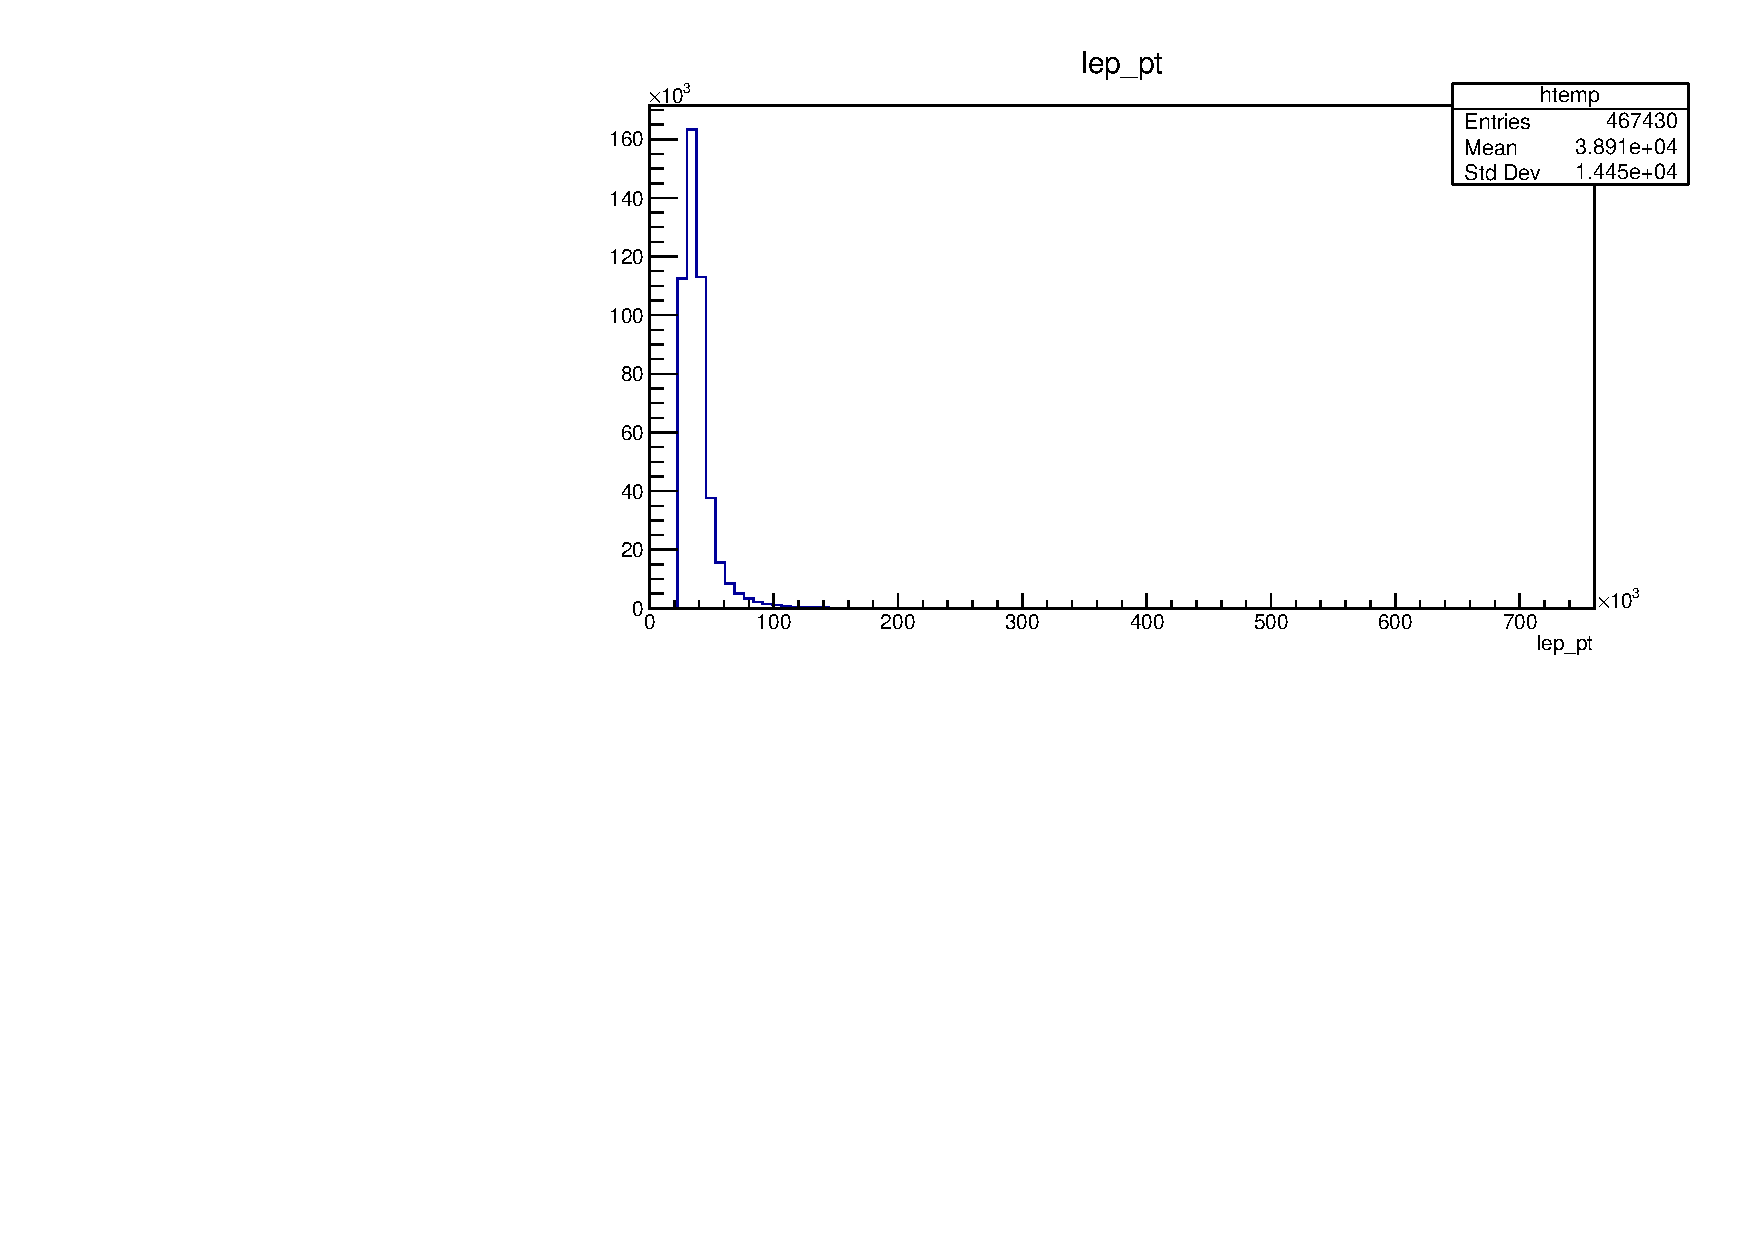
\includegraphics[width=0.8\textwidth]{content/graphics/question2_1/data_electron_6_pt.pdf}
  \caption{Histogramm des transversalen Impulses des Elektrons des Datentupels \textit{data.06.el}.}
  \label{fig:elec6pt}
\end{figure}
